% IUC Thesis & Dissertation Style Manual
% Sections 1-18 keep the structure of Edition 3.0; Section 19 covers the
% LaTeX template, GitHub, and AI tools.
%
% Build:  cd docs/style-manual && latexmk -xelatex iuc-style-manual.tex
\documentclass[11pt,a4paper]{article}

% ---------------------------------------------------------------------------
% Page, fonts, colours
% ---------------------------------------------------------------------------
\usepackage[a4paper,top=28mm,bottom=27mm,left=30mm,right=25mm,
  headheight=14pt,headsep=8mm,footskip=14mm]{geometry}
\usepackage{fontspec}
\setmainfont{Latin Modern Roman}
\setsansfont{Latin Modern Sans}
\setmonofont{Latin Modern Mono}
\IfFontExistsTF{Arial Narrow}{\newfontfamily\coverfont{Arial Narrow}}
  {\newfontfamily\coverfont{TeX Gyre Heros Cn}}
\IfFontExistsTF{Times New Roman}{\newfontfamily\tnr{Times New Roman}}
  {\newfontfamily\tnr{TeX Gyre Termes}}
\usepackage[british]{babel}
\usepackage[style=american]{csquotes}
\usepackage{xcolor}
\definecolor{iucpurple}{HTML}{5A2D82}
\definecolor{iucdeep}{HTML}{4D2470}
\definecolor{iucteal}{HTML}{2D6268}
\definecolor{iucgold}{HTML}{D9B96E}
\definecolor{iucbrown}{HTML}{7A5A1E}
\definecolor{iucrose}{HTML}{C58A73}
\definecolor{iuccream}{HTML}{F7F0E3}
\definecolor{iuclav}{HTML}{F2F0F5}
\definecolor{iuctealbg}{HTML}{E9EFEF}
\definecolor{iucgrey}{HTML}{5F5A66}
\definecolor{codebg}{HTML}{F7F5FA}

\usepackage{graphicx}
\graphicspath{{img/}}
\usepackage{pdfpages}
\usepackage{tikz}
\usetikzlibrary{positioning,arrows.meta,calc}
\usepackage[most]{tcolorbox}
\usepackage{listings}
\usepackage{enumitem}
\usepackage{array,tabularx,booktabs}
\usepackage{titlesec}
\usepackage{fancyhdr}
\usepackage{eso-pic}
\usepackage{amssymb,amsmath}
\usepackage{caption}
\usepackage{float}
\usepackage{needspace}
\newcommand\keepwithsample{\Needspace{200mm}}
\usepackage{microtype}
\usepackage[hidelinks]{hyperref}
\hypersetup{pdftitle={IUC Thesis and Dissertation Style Manual},
  pdfauthor={Innovative University College}}

\setlength\parindent{0pt}
\setlength\parskip{6pt}
\setlength\emergencystretch{3em}
\renewcommand\arraystretch{1.2}
\setlist{itemsep=5pt,topsep=4pt}
\setlist[itemize]{label=\textbullet,leftmargin=2.2em}
\setlist[enumerate]{leftmargin=2.2em}

\newcommand\repourl{https://github.com/fahimroslan/iucstyle_latex}
\newcommand\repo{\href{\repourl}{\texttt{github.com/fahimroslan/iucstyle\_latex}}}

% ---------------------------------------------------------------------------
% Headings and captions
% ---------------------------------------------------------------------------
\titleformat{\section}{\normalfont\Large\bfseries}{\thesection}{0.8em}{}
\titlespacing*{\section}{0pt}{18pt}{10pt}
\titleformat{\subsection}{\normalfont\large\bfseries}{\thesubsection}{0.8em}{}
\titlespacing*{\subsection}{0pt}{14pt}{6pt}
\titleformat{\subsubsection}{\normalfont\large\bfseries}{}{0pt}{}
\titlespacing*{\subsubsection}{0pt}{14pt}{6pt}
\setcounter{secnumdepth}{2}
\setcounter{tocdepth}{2}

\captionsetup{labelfont=bf,labelsep=colon,skip=6pt}
\captionsetup[table]{font=small,position=top}
\renewcommand\listfigurename{List of Figures and Page Samples}

% ---------------------------------------------------------------------------
% Running header and right-edge strip
% ---------------------------------------------------------------------------
\pagestyle{fancy}
\fancyhf{}
\fancyhead[L]{\small IUC Thesis and Dissertation Style Manual}
\fancyhead[R]{\small Institution-wide Standard}
\fancyfoot[C]{\thepage}
\renewcommand\headrulewidth{0.5pt}
\fancypagestyle{plain}{}

\newif\ifiucstrip \iucstriptrue
\AddToShipoutPictureBG{%
  \ifiucstrip
  \begin{tikzpicture}[remember picture,overlay,x=1mm,y=1mm]
    \shade[left color=white,right color=iucpurple!14]
      ($(current page.south east)+(-12,0)$) rectangle (current page.north east);
    \draw[iucpurple!35,line width=0.5pt]
      ($(current page.south east)+(-7,0)$) -- ($(current page.north east)+(-7,0)$);
    \draw[iucpurple!18,line width=2pt]
      ($(current page.south east)+(-4,0)$) -- ($(current page.north east)+(-4,0)$);
    \draw[iucrose,line width=0.8pt]
      ($(current page.south east)+(-7,24)$) -- ($(current page.south east)+(0,24)$);
  \end{tikzpicture}%
  \fi}

% ---------------------------------------------------------------------------
% Helpers
% ---------------------------------------------------------------------------
\newcommand\cmd[1]{\texttt{\textbackslash #1}}
\newcommand\file[1]{\texttt{#1}}
\newtcbox{\ui}{on line,colback=iuclav,colframe=iucpurple!40,boxrule=0.4pt,arc=2pt,
  boxsep=0pt,left=3pt,right=3pt,top=1.5pt,bottom=1pt,
  fontupper=\sffamily\small\bfseries\color{iucdeep}}
\newcommand\then{\,\textrightarrow\,}
\newcommand\cbox{$\square$}
\newcommand\thd[1]{\bfseries #1}

% Specification cards (Figure 1)
\newcommand\cardhead[1]{{\color{iucteal}\rule[-2.5pt]{1.8pt}{12pt}}\hspace{5pt}%
  {\sffamily\bfseries\color{iucpurple}#1}}
\newtcolorbox{card}[1]{enhanced,colback=iuclav,colframe=iucpurple!12,boxrule=0.5pt,
  arc=4pt,left=8pt,right=8pt,top=6pt,bottom=6pt,fontupper=\sffamily\small,
  before upper={\cardhead{#1}\par\smallskip}}

% Callouts and code (Section 19)
\tcbset{iucnote/.style={enhanced,boxrule=0pt,arc=2pt,left=9pt,right=9pt,top=6pt,
  bottom=6pt,before skip=8pt,after skip=8pt}}
\newtcolorbox{warnbox}[1][Important]{iucnote,colback=iuccream,
  borderline west={3pt}{0pt}{iucrose},
  before upper={\textbf{\sffamily\color{iucrose!75!black}#1.}\enspace}}
\newtcolorbox{promptbox}[1]{enhanced,colback=iuccream,colframe=iucgold,boxrule=0.6pt,
  arc=3pt,left=9pt,right=9pt,top=5pt,bottom=5pt,before skip=6pt,after skip=6pt,
  title={\sffamily\bfseries\small #1},colbacktitle=iucdeep,coltitle=white,
  toptitle=2pt,bottomtitle=2pt,fontupper=\itshape}
\lstdefinestyle{iuc}{language=[LaTeX]TeX,basicstyle=\ttfamily\small,
  texcsstyle=*\color{iucpurple}\bfseries,commentstyle=\color{iucgrey}\itshape,
  columns=fullflexible,keepspaces=true,showstringspaces=false,breaklines=true,
  upquote=true,
  moretexcs={textcite,parencite,addbibresource,printreferences,tablenote,
    figuresource,eqtitle,makecover,maketitlepage,makedeclaration,keywords,
    matricno,address,degree,degreeabbr,submissiondate,submissionyear,
    declarationdate,institution,toprule,midrule,bottomrule,mainmatter,frontmatter}}
\lstdefinestyle{plain}{basicstyle=\ttfamily\small,columns=fullflexible,
  keepspaces=true,breaklines=true,upquote=true}
% (no optional argument: a look-ahead for "[" would swallow the first line)
\tcbset{iuccode/.style={enhanced,listing only,colback=codebg,colframe=iucpurple!22,
  boxrule=0.5pt,arc=3pt,left=8pt,right=8pt,top=3pt,bottom=3pt,
  before skip=6pt,after skip=8pt}}
\newtcblisting{code}{iuccode,listing options={style=iuc}}
\newtcblisting{shell}{iuccode,colback=iucdeep,colframe=iucdeep,
  listing options={style=plain,basicstyle=\ttfamily\small\color{white}}}
\newtcblisting{prompttext}{iuccode,colback=iuccream,colframe=iucgold,
  listing options={style=plain}}

% ---------------------------------------------------------------------------
% Page samples at 50% (105 x 148.5 mm) with dimension labels and format notes
% ---------------------------------------------------------------------------
\newcommand\panelhead[2]{%
  \noindent{\sffamily\bfseries\color{iucpurple}\MakeUppercase{#1}}\hfill
  {\sffamily\bfseries\footnotesize\color{iucpurple}\MakeUppercase{#2}\hspace*{14mm}}\par
  \vspace{-3pt}{\color{iucgold!80!black}\rule{\linewidth}{0.6pt}}\par\vspace{4pt}}

\tikzset{dim/.style={{Stealth[length=1.4mm,width=1.2mm]}-{Stealth[length=1.4mm,width=1.2mm]},
    iucbrown,line width=0.4pt},
  dimlab/.style={font=\sffamily\tiny,text=iucgrey,fill=white,inner sep=1pt},
  guide/.style={iucbrown!60,dotted,line width=0.4pt}}

% Dimension labels and dashed text area.
% \pagedims{L}{T}{R}{B}{top label}{bottom label}{left label}{right label}
% L,T,R,B: text-area edges at 50% scale, in mm from the page's top-left corner.
\newcommand\pagedims[8]{%
  \draw[iucpurple!70,dashed,line width=0.4pt] (#1,-#2) rectangle (#3,-#4);
  \draw[guide] (#3,-#2) -- (110,-#2);
  \draw[guide] (#3,-#4) -- (110,-#4);
  \draw[guide] (105,0) -- (110,0);
  \draw[guide] (105,-148.5) -- (110,-148.5);
  \draw[dim] (108.5,0) -- node[dimlab,rotate=90]{#5} (108.5,-#2);
  \draw[dim] (108.5,-#4) -- node[dimlab,rotate=90]{#6} (108.5,-148.5);
  \draw[dim] (0,-152) -- node[dimlab]{#7} (#1,-152);
  \draw[dim] (#3,-152) -- node[dimlab]{#8} (105,-152);}
\newcommand\notespanel{\fill[iuclav,rounded corners=3pt] (112.5,0) rectangle (155,-148.5);}
% \samplepage{page}{L}{T}{R}{B}{top}{bottom}{left}{right}
\newcommand\samplepage[9]{%
  \node[anchor=north west,inner sep=0pt,draw=black,line width=0.4pt] at (0,0)
    {
\includegraphics[page=#1,width=105mm]{sample-pages}};
  \pagedims{#2}{#3}{#4}{#5}{#6}{#7}{#8}{#9}\notespanel}
% \fnote{number}{y}{title}{text}{target x,y}
\newcommand\fnote[5]{%
  \node[circle,fill=iucpurple,text=white,font=\sffamily\bfseries\scriptsize,
    inner sep=0pt,minimum size=4mm] (n#1) at (116,#2) {#1};
  \node[anchor=north west,text width=33.5mm,align=left,inner sep=0pt,
    font=\sffamily\scriptsize] at (119.5,#2+1.6) {\textbf{#3}\\[1pt]#4};
  \draw[iucpurple,line width=0.45pt,-{Stealth[length=1.8mm,width=1.4mm]}]
    (n#1.west) -- (#5);}
\newcommand\scalenote{%
  \node[anchor=north west,font=\sffamily\tiny,text=iucgrey] at (0,-156)
    {50\% scale: A4 page = 105 $\times$ 148.5 mm. Dimensions label full-size values.};}

% Standard settings for most samples: 30/25/38/25 mm
\newcommand\stdpage[1]{\samplepage{#1}{19}{15}{92.5}{136}{30 mm}{25 mm}{38 mm}{25 mm}}
\newcommand\openpage[1]{\samplepage{#1}{19}{20}{92.5}{136}{40 mm}{25 mm}{38 mm}{25 mm}}

\begin{document}

% ===========================================================================
% Cover
% ===========================================================================
\iucstripfalse

\includepdf[pages=1]{cover-front}
\iucstriptrue

\pagenumbering{roman}
\tableofcontents
\clearpage
\listoftables
\clearpage
\listoffigures
\clearpage
\pagenumbering{arabic}

% ===========================================================================
\section{Purpose of this manual}
% ===========================================================================

This manual is the institution-wide formatting standard for all Innovative
University College (IUC) master's and doctoral theses, dissertations, and
research projects. It applies to every study mode listed in Table~\ref{tab:words}.

This manual is the sole authority for manuscript formatting at IUC. Its rules
apply across all faculties and programmes, and no separate formatting guide is
required. APA 7th edition governs citations and references; the IUC rules in
this manual govern how the manuscript is presented.

IUC provides a LaTeX template that applies these rules automatically.
Candidates who use it should keep its preset margins, headings, page
numbering, and formatting. Section~\ref{sec:latex} explains how to obtain and use
the template, including with GitHub and AI tools.

\subsubsection*{Reading the illustrations}

Each page sample is a full A4 page produced by the template, reduced uniformly
to 50\%. Fonts, line spacing, margins, and content positions scale together.
Dashed lines mark the text area. Numbered notes sit outside the page, with
arrows pointing to the matching feature; the arrows are annotations, not part
of the manuscript. Print this manual at actual size (100\%) to preserve the
stated scale. The template's sample manuscript shows the same pages at full
size (Section~\ref{sec:latex}).

\subsection{Candidate responsibility}

The template sets the layout. Candidates remain responsible for accuracy,
academic quality, and the following checks:

\begin{itemize}
  \item personal, programme, degree, and submission details;
  \item the approved thesis or dissertation title;
  \item the compulsory minimum word count, and concise abstracts;
  \item the required citation and reference style;
  \item permission to use copyrighted material, where necessary;
  \item every table, figure, equation, citation, and appendix;
  \item the printing, binding, and PDF-submission rules in this manual; and
  \item every page of the final PDF.
\end{itemize}

% ===========================================================================
\section{Template specifications at a glance}
% ===========================================================================

\begin{figure}[htbp]
\begin{tcbraster}[raster columns=2,raster equal height=rows,raster column skip=9pt,
  raster row skip=9pt]
\begin{card}{Manuscript and paper}
  Formal thesis or dissertation.\par
  \textbf{A4:} 210~mm $\times$ 297~mm.
\end{card}
\begin{card}{Page margins}
  \textbf{Standard:} top 30~mm; bottom 25~mm; left 38~mm; right 25~mm.\par
  \textbf{Chapter opening:} top 40~mm; other margins unchanged.
\end{card}
\begin{card}{Body and paragraphs}
  \textbf{Times New Roman, 12~pt} body text, double-spaced.\par
  \textbf{2~em} first-line indent; \textbf{6~pt} after each paragraph.
\end{card}
\begin{card}{Heading treatment}
  \textbf{Chapters:} bold uppercase; title centred beneath the chapter number.\par
  \textbf{Sections:} bold, left aligned, numbered by chapter.
\end{card}
\begin{card}{Page numbering}
  \textbf{Front matter:} lowercase Roman numerals.\par
  \textbf{Main text:} Arabic numerals, starting at 1.\par
  Page numbers centred at the bottom.
\end{card}
\begin{card}{Sources and appendices}
  \textbf{Citations:} APA 7th edition author--year style.\par
  \textbf{Appendices:} lettered: Appendix A, Appendix B, and so on.
\end{card}
\end{tcbraster}
\caption{Visual summary of template specifications.}
\label{fig:glance}
\end{figure}

\textbf{Paper size.} Use A4 (210~$\times$~297~mm) for the manuscript and the
final PDF. Print at actual size, without scaling.

% ===========================================================================
\section{Word-count requirements}\label{sec:words}
% ===========================================================================

The minimum word counts in Table~\ref{tab:words} are compulsory. The advisory
maximums are for planning only: there is no fixed upper limit, and no exemption
is needed to exceed them.

\begin{table}[htbp]
\caption{Institution-wide minimum and advisory word counts.}
\label{tab:words}
\small
\begin{tabularx}{\textwidth}{@{}p{34mm}X>{\raggedleft\arraybackslash}p{24mm}>{\raggedleft\arraybackslash}p{24mm}@{}}
\toprule
\thd{Level} & \thd{Mode} & \thd{Compulsory minimum} & \thd{Advisory maximum} \\
\midrule
Master   & Coursework + Research Project & 10,000 & 30,000 \\
Master   & Mixed Mode                    & 25,000 & 50,000 \\
Master   & Full Research                 & 40,000 & 60,000 \\
Doctoral / Professional Doctorate & Coursework + Dissertation & 40,000 & 60,000 \\
PhD      & Full Research                 & 70,000 & 100,000 \\
\bottomrule
\end{tabularx}
\par\smallskip\raggedright\small\textit{Note.} These requirements depend on the
study mode, regardless of programme or discipline.
\end{table}

\subsection{Counting scope}

Count the chapter body text from the first chapter to the last, including
headings and quotations. Exclude the front matter, abstracts, table and figure
content, captions, references, and appendices.

The LaTeX template does not count words or enforce limits.

\subsection{Abstracts and final verification}

Neither the English abstract nor the Malay \emph{Abstrak} has a fixed word
limit. Each must concisely state the objectives, methods, findings, and
conclusion. Keywords below each abstract are optional.

Before submission, check that the chapter body text meets the compulsory
minimum for the study mode. Exceeding the advisory maximum is permitted.

% ===========================================================================
\section{Required order of the manuscript}
% ===========================================================================

Arrange the manuscript in the order shown in Figure~\ref{fig:order}.

\begin{figure}[htbp]
\centering
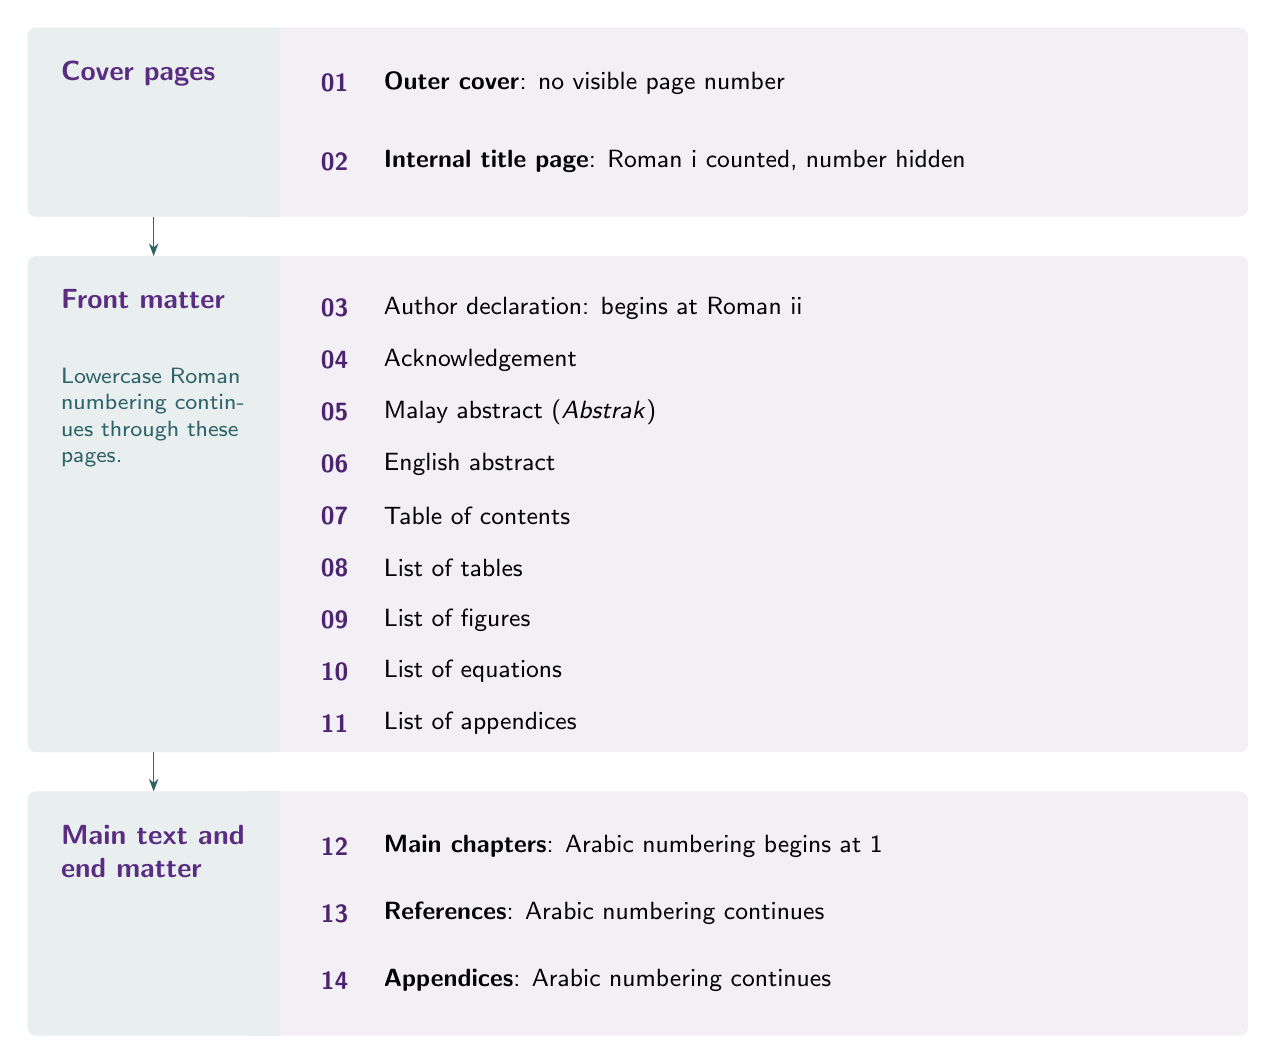
\begin{tikzpicture}[x=1mm,y=1mm,
  lab/.style={anchor=north west,font=\sffamily\bfseries\color{iucpurple},align=left,text width=26mm},
  sub/.style={anchor=north west,font=\sffamily\footnotesize\color{iucteal},align=left,text width=24mm},
  num/.style={anchor=west,font=\sffamily\bfseries\small\color{iucdeep}},
  item/.style={anchor=west,font=\sffamily\small,align=left},
  arr/.style={-{Stealth[length=1.6mm]},draw=iucteal,line width=0.5pt}]
  % Cover pages
  \fill[iuclav,rounded corners=3pt] (0,0) rectangle (155,-24);
  \fill[iuctealbg,rounded corners=3pt] (0,0) rectangle (32,-24);
  \fill[iuctealbg] (28,0) rectangle (32,-24);
  \node[lab] at (3,-3) {Cover pages};
  \node[num] at (36,-7) {01}; \node[item] at (44,-7) {\textbf{Outer cover}: no visible page number};
  \node[num] at (36,-17) {02}; \node[item] at (44,-17) {\textbf{Internal title page}: Roman i counted, number hidden};
  \draw[arr] (16,-24) -- (16,-29);
  % Front matter
  \fill[iuclav,rounded corners=3pt] (0,-29) rectangle (155,-92);
  \fill[iuctealbg,rounded corners=3pt] (0,-29) rectangle (32,-92);
  \fill[iuctealbg] (28,-29) rectangle (32,-92);
  \node[lab] at (3,-32) {Front matter};
  \node[sub] at (3,-42) {Lowercase Roman numbering continues through these pages.};
  \foreach \n/\t [count=\k] in {03/{Author declaration: begins at Roman ii},04/Acknowledgement,
      05/{Malay abstract (\emph{Abstrak})},06/English abstract,07/Table of contents,
      08/List of tables,09/List of figures,10/List of equations,11/List of appendices}
    { \node[num] at (36,-29-\k*6.6) {\n}; \node[item] at (44,-29-\k*6.6) {\t}; }
  \draw[arr] (16,-92) -- (16,-97);
  % Main text
  \fill[iuclav,rounded corners=3pt] (0,-97) rectangle (155,-128);
  \fill[iuctealbg,rounded corners=3pt] (0,-97) rectangle (32,-128);
  \fill[iuctealbg] (28,-97) rectangle (32,-128);
  \node[lab] at (3,-100) {Main text and end matter};
  \node[num] at (36,-104) {12}; \node[item] at (44,-104) {\textbf{Main chapters}: Arabic numbering begins at 1};
  \node[num] at (36,-112.5) {13}; \node[item] at (44,-112.5) {\textbf{References}: Arabic numbering continues};
  \node[num] at (36,-121) {14}; \node[item] at (44,-121) {\textbf{Appendices}: Arabic numbering continues};
\end{tikzpicture}
\caption{Manuscript assembly sequence and pagination transitions; read from top to bottom.}
\label{fig:order}
\end{figure}

Keep this order. Omit any list that has no entries. A dedication is optional
and follows the acknowledgement; a list of abbreviations and a glossary may
follow the list of appendices when needed. Use the same front-matter format and
Roman pagination for these pages.

% ===========================================================================
\section{Cover and title-page information}
% ===========================================================================

Check these details against your official registration and approved research
records:

\begin{itemize}
  \item the complete, approved thesis or dissertation title;
  \item the candidate's full registered name;
  \item the name of the institution;
  \item the department, faculty, or academic unit, if included;
  \item the complete name of the degree;
  \item the month and year of submission;
  \item the declaration date;
  \item the matriculation or candidate number; and
  \item the candidate's address on the declaration page.
\end{itemize}

\textbf{Page samples.} Each A4 page is shown at 105~$\times$~148.5~mm (50\%).
Dimension labels show full-size millimetres. Page numbers and contents entries
come from the same compiled sample manuscript. Annotation text is enlarged for
readability.

\subsection{Outer cover}

The outer cover shows the title, the registered candidate name, and the
institution name, in \textbf{18-point Arial Narrow, bold uppercase,
single-spaced, with gold hot stamping}. Centre the title at the top, the name
in the middle, and the institution near the bottom. Break long titles into
balanced lines, and keep each name on one line where possible.

The cover uses special margins: 60~mm at the top, 40~mm at the bottom, 40~mm on
the left, and 25~mm on the right. No page number is shown.

The final hardbound cover and spine are colour-coded by award level:

\begin{itemize}
  \item \textbf{Doctoral level (PhD and professional doctorates):} black
        hardbound cover and spine with gold lettering.
  \item \textbf{Master's level (all study modes):} purple hardbound cover and
        spine with gold lettering.
\end{itemize}

Use the specified colour for the front cover, back cover, and spine. Keep the
gold lettering clear, durable, and consistent. The illustration uses sample
details; the cover page in the submitted PDF is white with black lettering.

\begin{figure}[H]
\panelhead{Outer cover}{Format notes}
\centering
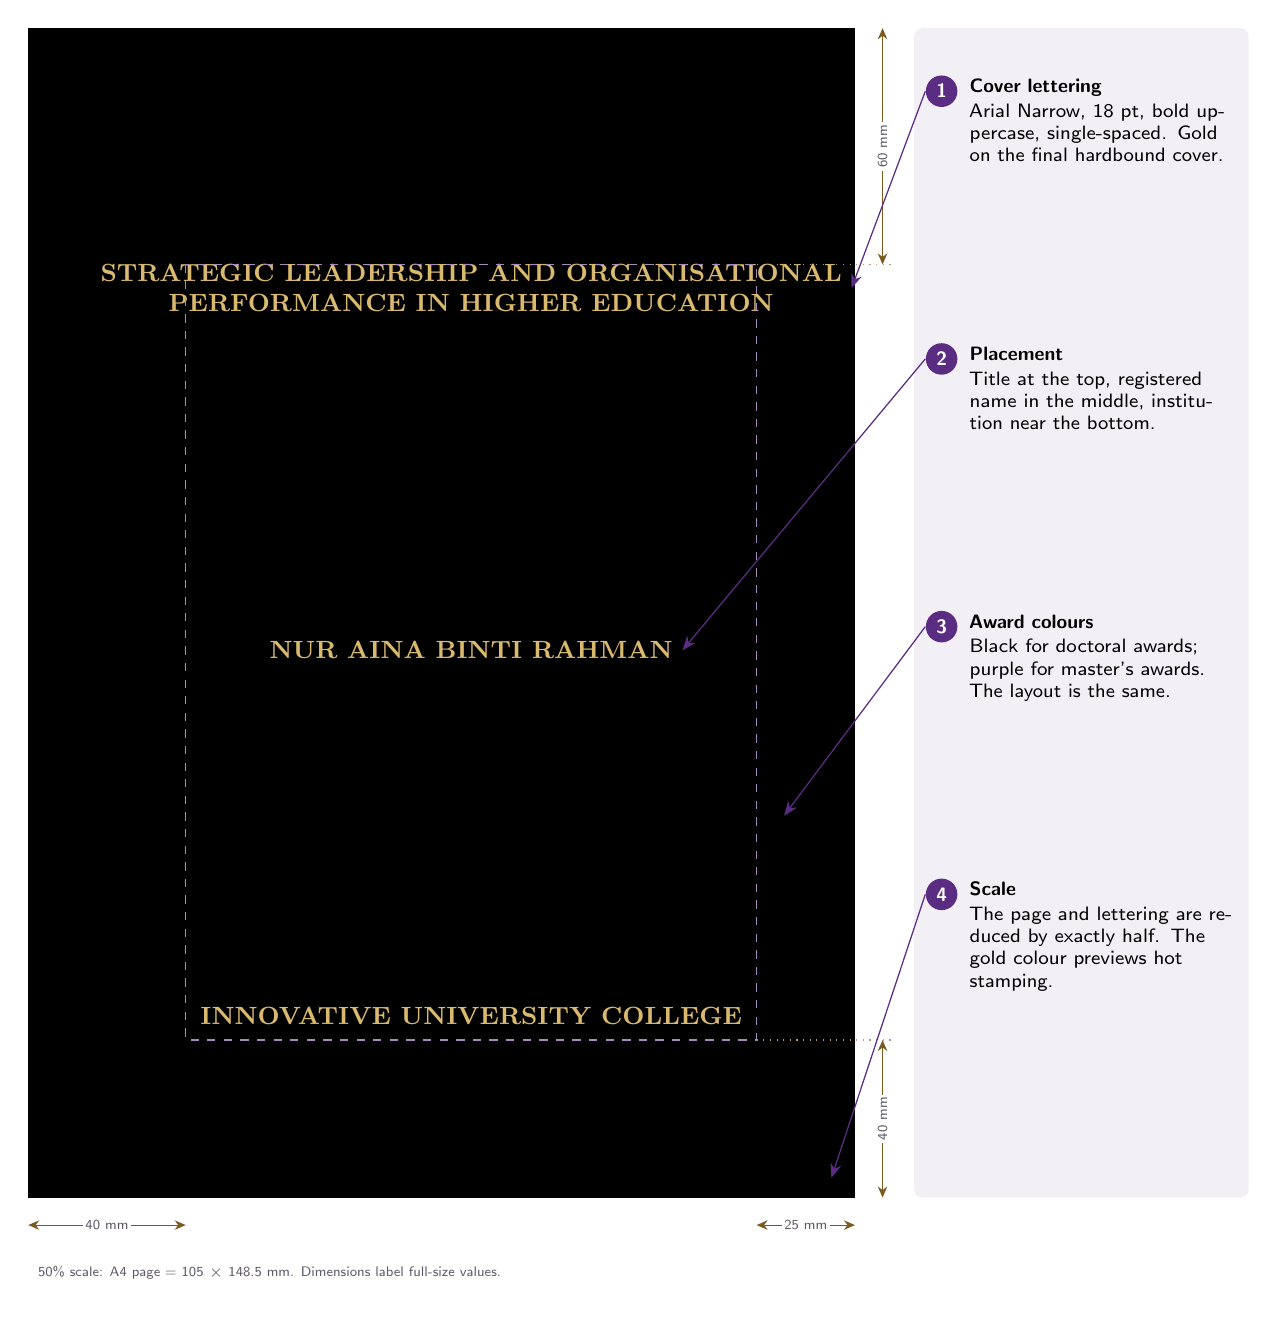
\begin{tikzpicture}[x=1mm,y=1mm]
  \fill[black] (0,0) rectangle (105,-148.5);
  \node[text=iucgold,font=\coverfont\bfseries\fontsize{9}{10.8}\selectfont,align=center]
    (ct) at (56.25,-33) {STRATEGIC LEADERSHIP AND ORGANISATIONAL\\PERFORMANCE IN HIGHER EDUCATION};
  \node[text=iucgold,font=\coverfont\bfseries\fontsize{9}{10.8}\selectfont] (cn)
    at (56.25,-79) {NUR AINA BINTI RAHMAN};
  \node[text=iucgold,font=\coverfont\bfseries\fontsize{9}{10.8}\selectfont] (ci)
    at (56.25,-125.5) {INNOVATIVE UNIVERSITY COLLEGE};
  \draw[iucpurple!55,dashed,line width=0.4pt] (20,-30) rectangle (92.5,-128.5);
  \draw[guide] (92.5,-30) -- (110,-30);
  \draw[guide] (92.5,-128.5) -- (110,-128.5);
  \draw[dim] (108.5,0) -- node[dimlab,rotate=90]{60 mm} (108.5,-30);
  \draw[dim] (108.5,-128.5) -- node[dimlab,rotate=90]{40 mm} (108.5,-148.5);
  \draw[dim] (0,-152) -- node[dimlab]{40 mm} (20,-152);
  \draw[dim] (92.5,-152) -- node[dimlab]{25 mm} (105,-152);
  \notespanel
  \fnote{1}{-8}{Cover lettering}{Arial Narrow, 18~pt, bold uppercase,
    single-spaced. Gold on the final hardbound cover.}{ct.east}
  \fnote{2}{-42}{Placement}{Title at the top, registered name in the middle,
    institution near the bottom.}{cn.east}
  \fnote{3}{-76}{Award colours}{Black for doctoral awards; purple for master's
    awards. The layout is the same.}{96,-100}
  \fnote{4}{-110}{Scale}{The page and lettering are reduced by exactly half. The
    gold colour previews hot stamping.}{102,-146}
  \scalenote
\end{tikzpicture}
\caption{Doctoral hardbound outer-cover sample; the master's version uses the same layout in purple.}
\label{fig:cover}
\end{figure}

\subsubsection*{Hardbound spine information}

Leave \textbf{60~mm clear at each end of the spine}. Set the registered name
vertically on one line, followed by the degree abbreviation and the submission
year. Use the abbreviation of the registered award, such as MBA, MSc, PhD, or
DBA; split a long award name across tightly stacked lines. Start the name at
the upper printable boundary and end the year at the lower boundary.

Use \textbf{16-point Arial Narrow, bold uppercase, with gold hot stamping},
reading from top to bottom. Centre the lettering within the spine width
confirmed by the binder. Match all details to the title page and official
records. The illustration uses a sample name and year.

\begin{figure}[H]
\panelhead{Hardbound spines}{Format notes}
\centering
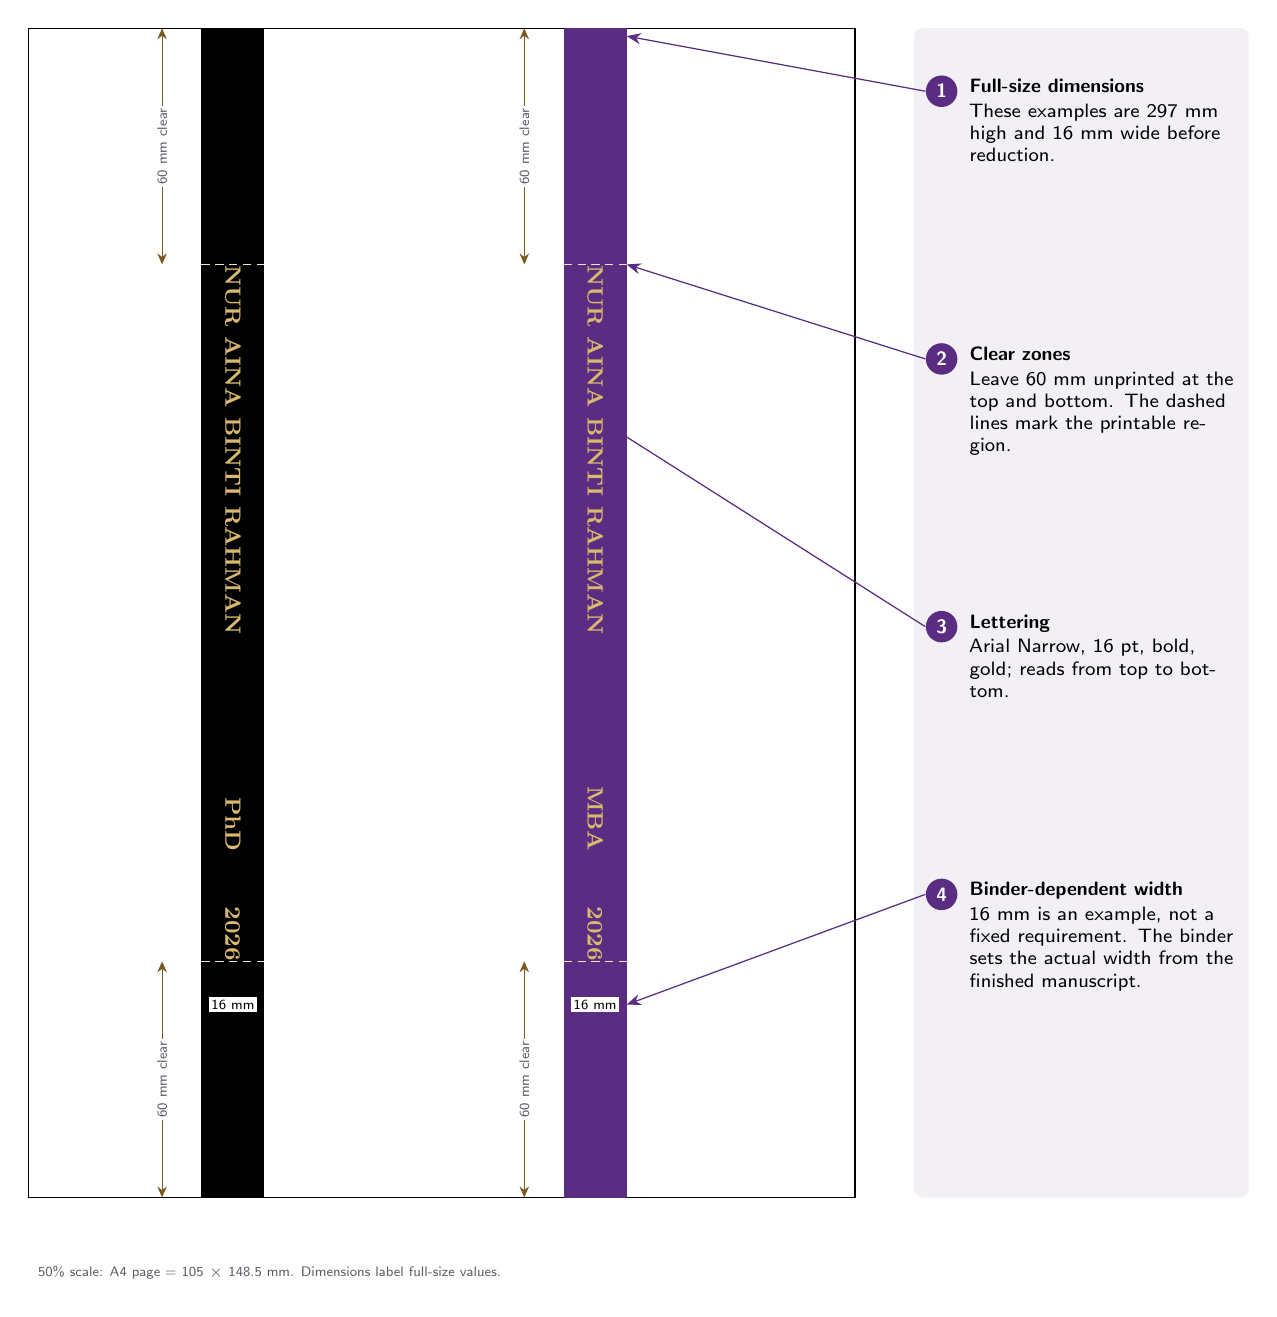
\begin{tikzpicture}[x=1mm,y=1mm]
  \draw[line width=0.4pt] (0,0) rectangle (105,-148.5);
  \foreach \x/\col/\deg/\k in {26/black/PhD/a,72/iucpurple/MBA/b} {
    \fill[\col] (\x-4,0) rectangle (\x+4,-148.5);
    \draw[white!60!iucgold,densely dashed,line width=0.3pt] (\x-4,-30) -- (\x+4,-30);
    \draw[white!60!iucgold,densely dashed,line width=0.3pt] (\x-4,-118.5) -- (\x+4,-118.5);
    \node[rotate=-90,anchor=west,inner sep=0pt,text=iucgold,
      font=\coverfont\bfseries\fontsize{8}{8}\selectfont] (nm\k) at (\x,-30) {NUR AINA BINTI RAHMAN};
    \node[rotate=-90,anchor=east,inner sep=0pt,text=iucgold,
      font=\coverfont\bfseries\fontsize{8}{8}\selectfont] (yr\k) at (\x,-118.5) {\deg\hspace{7mm}2026};
    \draw[dim] (\x-9,0) -- node[dimlab,rotate=90]{60 mm clear} (\x-9,-30);
    \draw[dim] (\x-9,-118.5) -- node[dimlab,rotate=90]{60 mm clear} (\x-9,-148.5);
    \node[fill=white,font=\sffamily\tiny,inner sep=1pt] at (\x,-124) {16 mm};
  }
  \notespanel
  \fnote{1}{-8}{Full-size dimensions}{These examples are 297~mm high and 16~mm
    wide before reduction.}{76,-1}
  \fnote{2}{-42}{Clear zones}{Leave 60~mm unprinted at the top and bottom. The
    dashed lines mark the printable region.}{76,-30}
  \fnote{3}{-76}{Lettering}{Arial Narrow, 16~pt, bold, gold; reads from top to
    bottom.}{73,-50}
  \fnote{4}{-110}{Binder-dependent width}{16~mm is an example, not a fixed
    requirement. The binder sets the actual width from the finished
    manuscript.}{76,-124}
  \scalenote
\end{tikzpicture}
\caption{Spine examples at 50\% scale; the 16~mm full-size width is illustrative.}
\label{fig:spine}
\end{figure}

\subsection{Internal title page}

The internal title page contains:

\begin{enumerate}
  \item the approved thesis or dissertation title;
  \item the candidate's name;
  \item the statement that the work is submitted in partial fulfilment of the degree;
  \item the full degree title;
  \item the institution name; and
  \item the month and year of submission.
\end{enumerate}

Set the title in 14-point Times New Roman, bold uppercase and single-spaced.
Set the rest in 12-point Times New Roman: the name in regular type with each
word capitalised; the submission statement and date in sentence case; the degree
in bold uppercase; and the institution in regular uppercase. Use the
outer-cover margins. The title page counts as Roman page~i, but the number is
not shown.

Break long titles into balanced, single-spaced lines. Keep the approved wording
and abbreviations, and match the title and name to the outer cover.

\begin{figure}[H]
\panelhead{Internal title page}{Format notes}
\centering
\begin{tikzpicture}[x=1mm,y=1mm]
  \samplepage{1}{20}{30}{92.5}{128.5}{60 mm}{40 mm}{40 mm}{25 mm}
  \fnote{1}{-8}{Title}{Times New Roman, 14~pt, bold uppercase, single-spaced.}{87,-31.5}
  \fnote{2}{-42}{Margins}{60~mm top, 40~mm bottom and left, 25~mm right at full
    size.}{92.5,-45}
  \fnote{3}{-76}{Other text}{Times New Roman, 12~pt. Name and institution
    regular; degree title bold uppercase.}{80,-81.5}
  \fnote{4}{-110}{Pagination}{Counted as Roman page~i; the number is not
    printed.}{56,-140}
  \scalenote
\end{tikzpicture}
\caption{Internal title-page sample at 50\% scale.}
\label{fig:title}
\end{figure}

\clearpage
% ===========================================================================
\section{Front matter}
% ===========================================================================

Start each front-matter component on a new page. Use 12-point Times New Roman
with centred, bold uppercase headings. Unless stated otherwise, use regular,
sentence-case, justified, single-spaced text.

\subsection{Author declaration}

The declaration confirms that the work is the candidate's own and that all
sources are acknowledged.

Use the front-matter format. Place the date on the left, and the signature,
name, matriculation number, and address on the right. Use the exact declaration
shown below and complete all details.

\begin{figure}[H]
\panelhead{Author declaration}{Format notes}
\centering
\begin{tikzpicture}[x=1mm,y=1mm]
  \stdpage{2}
  \fnote{1}{-8}{Heading}{Times New Roman, 12~pt, bold uppercase, centred.}{69,-16.3}
  \fnote{2}{-42}{Declaration}{Times New Roman, 12~pt, single-spaced and
    justified. Keep the required wording.}{92.5,-23}
  \fnote{3}{-76}{Details}{Date on the left; signature and candidate details on
    the right.}{87.5,-40}
  \fnote{4}{-110}{Pagination}{Roman page~ii. Page numbers are centred at the
    bottom.}{57,-141}
  \scalenote
\end{tikzpicture}
\caption{Author-declaration sample.}
\label{fig:decl}
\end{figure}

\subsection{Acknowledgement}

Briefly acknowledge academic, financial, technical, and personal support in a
formal tone. Include funders, research sites, and specialist contributors where
applicable.

Write in paragraphs using 12-point Times New Roman, sentence case, justified
alignment, and single spacing.

\begin{figure}[H]
\panelhead{Acknowledgement}{Format notes}
\centering
\begin{tikzpicture}[x=1mm,y=1mm]
  \stdpage{3}
  \fnote{1}{-8}{Heading}{Centred, bold uppercase, 12~pt.}{68,-16.3}
  \fnote{2}{-42}{Text}{Times New Roman, 12~pt, single-spaced and justified.}{92.5,-26}
  \fnote{3}{-76}{Content}{Acknowledge academic, financial, technical, and
    personal support briefly.}{60,-31}
  \fnote{4}{-110}{Pagination}{Continue lowercase Roman page numbering.}{57.5,-141}
  \scalenote
\end{tikzpicture}
\caption{Acknowledgement sample.}
\label{fig:ack}
\end{figure}

\subsection{Malay abstract: \emph{Abstrak}}

Place the Malay abstract before the English version. Both must report the same
study, findings, and conclusions, with matching terms, names, abbreviations,
and numbers.

Each abstract must summarise:

\begin{itemize}
  \item the research context or problem;
  \item the study objectives;
  \item the method or research design;
  \item the main findings; and
  \item the main conclusion or contribution.
\end{itemize}

There is no fixed word limit for either abstract, and keywords are optional.
Ensure that both language versions are accurate.

\begin{figure}[H]
\panelhead{Abstrak}{Format notes}
\centering
\begin{tikzpicture}[x=1mm,y=1mm]
  \stdpage{4}
  \fnote{1}{-8}{Heading}{ABSTRAK: centred, bold uppercase, 12~pt.}{61.5,-16.3}
  \fnote{2}{-42}{Text}{Times New Roman, 12~pt, single-spaced and justified.}{92.5,-30}
  \fnote{3}{-76}{Content}{Malay version first. Match the English abstract in
    meaning. No fixed word limit; keywords are optional.}{75.5,-48.8}
  \fnote{4}{-110}{Pagination}{Continue lowercase Roman page numbering.}{57.5,-141}
  \scalenote
\end{tikzpicture}
\caption{Malay abstract (\emph{Abstrak}) sample.}
\label{fig:abstrak}
\end{figure}

\subsection{English abstract}

The English abstract follows the Malay version. Summarise the research clearly,
without adding claims that are absent from the thesis. Avoid citations unless
they are required.

Use few abbreviations, and define each at first use. Check both abstracts side
by side for consistency. Keep the abstract concise; optional keywords appear
below it.

\begin{figure}[H]
\panelhead{Abstract}{Format notes}
\centering
\begin{tikzpicture}[x=1mm,y=1mm]
  \stdpage{5}
  \fnote{1}{-8}{Heading}{ABSTRACT: centred, bold uppercase, 12~pt.}{62,-16.3}
  \fnote{2}{-42}{Text}{Times New Roman, 12~pt, single-spaced and justified.}{92.5,-30}
  \fnote{3}{-76}{Content}{English version follows the Abstrak. No fixed word
    limit; keywords are optional.}{75.5,-43.8}
  \fnote{4}{-110}{Pagination}{Continue lowercase Roman page numbering.}{57,-141}
  \scalenote
\end{tikzpicture}
\caption{English abstract sample.}
\label{fig:abstract}
\end{figure}

\subsection{Table of contents}

List the front matter, chapters, sections, references, and appendices.
Subsections and lower headings are not listed.

Use chapter entries such as \texttt{CHAPTER 1: INTRODUCTION}. Main chapter
headings have no page number in the contents; all other entries show one. The
template generates the entries, so do not edit them by hand. Use single spacing,
and match every title exactly to the manuscript.

\begin{figure}[H]
\panelhead{Table of contents}{Format notes}
\centering
\begin{tikzpicture}[x=1mm,y=1mm]
  \stdpage{6}
  \fnote{1}{-8}{Entries}{Times New Roman, 12~pt, single-spaced. Entries come
    from the compiled manuscript.}{93,-28}
  \fnote{2}{-42}{Chapter entries}{Main chapter headings have no displayed page
    number.}{47.5,-52.7}
  \fnote{3}{-76}{Depth}{Chapters and sections are included; subsections are
    omitted.}{45,-93.4}
  \fnote{4}{-110}{Other entries}{Page numbers are shown for front matter,
    sections, references, and appendices.}{93,-103.5}
  \scalenote
\end{tikzpicture}
\caption{Table-of-contents sample.}
\label{fig:toc}
\end{figure}

\subsection{Lists of tables, figures, equations, and appendices}

Start each list on a new page. Use single spacing, and match the numbers and
captions or titles to the manuscript. Omit a list when the manuscript has no
corresponding items.

\keepwithsample
\textbf{List of tables.} Include every numbered table, with its caption and
page number, in manuscript order.

\begin{figure}[H]
\panelhead{List of tables}{Format notes}
\centering
\begin{tikzpicture}[x=1mm,y=1mm]
  \stdpage{7}
  \fnote{1}{-8}{Heading}{Centred, bold uppercase, 12~pt.}{64.5,-16.3}
  \fnote{2}{-42}{Columns}{Match table numbers and captions to the manuscript.
    Align page numbers at the right.}{93,-26}
  \fnote{3}{-76}{Entries}{Times New Roman, 12~pt, single-spaced. Include every
    numbered table.}{45,-26.5}
  \fnote{4}{-110}{Pagination}{Continue lowercase Roman page numbering. Omit the
    list when there are no entries.}{57,-141}
  \scalenote
\end{tikzpicture}
\caption{List-of-tables sample.}
\label{fig:lot}
\end{figure}

\keepwithsample
\textbf{List of figures.} Include every numbered figure, with its caption and
page number, in manuscript order.

\begin{figure}[H]
\panelhead{List of figures}{Format notes}
\centering
\begin{tikzpicture}[x=1mm,y=1mm]
  \stdpage{8}
  \fnote{1}{-8}{Heading}{Centred, bold uppercase, 12~pt.}{65,-16.3}
  \fnote{2}{-42}{Columns}{Match figure numbers and captions to the manuscript.
    Align page numbers at the right.}{93,-26}
  \fnote{3}{-76}{Entries}{Times New Roman, 12~pt, single-spaced. Include every
    numbered figure.}{50,-26.5}
  \fnote{4}{-110}{Pagination}{Continue lowercase Roman page numbering. Omit the
    list when there are no entries.}{57.5,-141}
  \scalenote
\end{tikzpicture}
\caption{List-of-figures sample.}
\label{fig:lof}
\end{figure}

\keepwithsample
\textbf{List of equations.} Include every numbered equation, with a short
descriptive title and its page number. Do not reproduce the expression itself.

\begin{figure}[H]
\panelhead{List of equations}{Format notes}
\centering
\begin{tikzpicture}[x=1mm,y=1mm]
  \stdpage{9}
  \fnote{1}{-8}{Heading}{Centred, bold uppercase, 12~pt.}{66.5,-16.3}
  \fnote{2}{-42}{Page numbers}{Align the page number at the right. Keep entries
    single-spaced.}{93,-24.5}
  \fnote{3}{-76}{Entries}{Include every numbered equation with a short
    descriptive title and page number.}{48,-24.8}
  \fnote{4}{-110}{Pagination}{Continue lowercase Roman page numbering. Omit the
    list when there are no entries.}{57,-141}
  \scalenote
\end{tikzpicture}
\caption{List-of-equations sample.}
\label{fig:loe}
\end{figure}

\keepwithsample
\textbf{List of appendices.} Include each appendix letter, title, and starting
page number.

\begin{figure}[H]
\panelhead{List of appendices}{Format notes}
\centering
\begin{tikzpicture}[x=1mm,y=1mm]
  \stdpage{10}
  \fnote{1}{-8}{Heading}{Centred, bold uppercase, 12~pt.}{67,-16.3}
  \fnote{2}{-42}{Page numbers}{Align the starting page number at the right.
    Keep entries single-spaced.}{93,-24.5}
  \fnote{3}{-76}{Entries}{Include each appendix letter, title, and starting
    page number.}{52,-24.8}
  \fnote{4}{-110}{Pagination}{Continue lowercase Roman page numbering. Omit the
    list when there are no entries.}{56.5,-141}
  \scalenote
\end{tikzpicture}
\caption{List-of-appendices sample.}
\label{fig:loa}
\end{figure}

\clearpage
% ===========================================================================
\section{Organization of the main text}
% ===========================================================================

Start the main text at Arabic page~1, and start each chapter on a new page. The
template provides five chapters:

\begin{enumerate}
  \item Introduction
  \item Literature Review
  \item Methodology
  \item Data Analysis
  \item Discussion and Conclusion
\end{enumerate}

This five-chapter structure is a flexible default for all study modes. Combine
or split chapters to suit the research, while covering the elements below.

Arrange the chapters logically to explain:

\begin{itemize}
  \item the research problem and its significance;
  \item the objectives, questions, or hypotheses;
  \item the relevant scholarly context;
  \item the method used to conduct the study;
  \item the evidence or results obtained;
  \item the interpretation of those results; and
  \item the study's conclusions, limitations, implications, and recommendations.
\end{itemize}

Use short, descriptive chapter titles. A chapter may begin with a brief
introduction or proceed directly to its first section.

\begin{figure}[H]
\panelhead{Chapter opening}{Format notes}
\centering
\begin{tikzpicture}[x=1mm,y=1mm]
  \openpage{11}
  \fnote{1}{-8}{Chapter heading}{Times New Roman, 12~pt, bold uppercase,
    centred. Top margin: 40~mm.}{62.5,-21.5}
  \fnote{2}{-42}{Section headings}{12~pt, bold, left aligned. 24~pt before and
    12~pt after.}{33,-35}
  \fnote{3}{-76}{Body text}{Times New Roman, 12~pt, justified and
    double-spaced.}{92.5,-62.5}
  \fnote{4}{-110}{Paragraphs}{2~em first-line indent; 6~pt after each
    paragraph.}{23.5,-94}
  \scalenote
\end{tikzpicture}
\caption{Chapter-opening sample.}
\label{fig:chapter}
\end{figure}

\keepwithsample
\textbf{Continuation pages.} Use the standard 30~mm top margin, and keep all
content within the text area.

\begin{figure}[H]
\panelhead{Chapter continuation}{Format notes}
\centering
\begin{tikzpicture}[x=1mm,y=1mm]
  \stdpage{12}
  \fnote{1}{-8}{Top margin}{Continuation pages use the standard 30~mm top
    margin.}{92.5,-15}
  \fnote{2}{-42}{Headings}{Keep section and subsection styles consistent with
    the chapter opening.}{40.5,-37}
  \fnote{3}{-76}{Body text}{Times New Roman, 12~pt, double-spaced; 2~em
    first-line indent and 6~pt after paragraphs.}{92.5,-47}
  \fnote{4}{-110}{Pagination}{Continue Arabic numbering. The footer baseline is
    12.5~mm above the bottom edge.}{57,-141}
  \scalenote
\end{tikzpicture}
\caption{Chapter-continuation sample.}
\label{fig:continuation}
\end{figure}

\clearpage
% ===========================================================================
\section{Page layout}
% ===========================================================================

\subsection{Standard margins}

Figure~\ref{fig:margins} compares the standard and chapter-opening margins.
Only the top margin changes.

\begin{figure}[htbp]
\centering
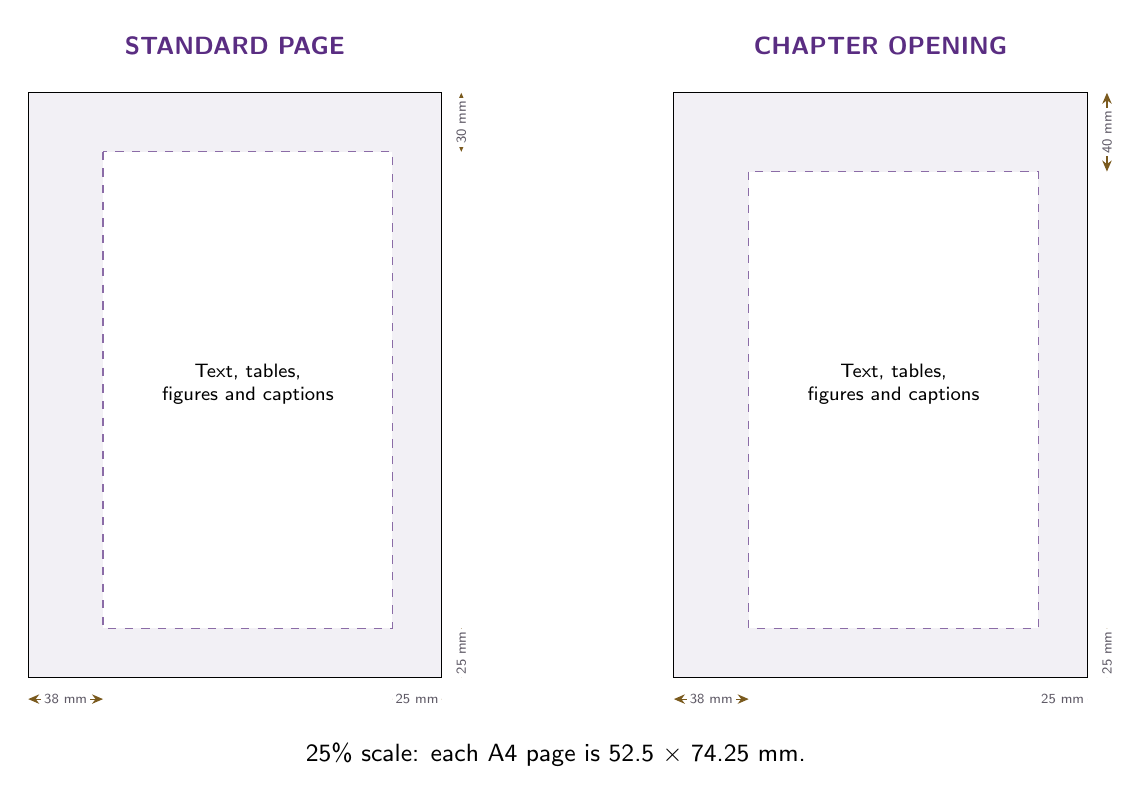
\begin{tikzpicture}[x=1mm,y=1mm]
  \foreach \x/\lab/\top in {0/Standard page/7.5,82/Chapter opening/10} {
    \begin{scope}[shift={(\x,0)}]
      \node[font=\sffamily\bfseries\small,text=iucpurple] at (26.25,6) {\MakeUppercase{\lab}};
      \fill[iuclav] (0,0) rectangle (52.5,-74.25);
      \draw[line width=0.4pt] (0,0) rectangle (52.5,-74.25);
      \fill[white] (9.5,-\top) rectangle (46.25,-68);
      \draw[iucpurple!70,dashed,line width=0.4pt] (9.5,-\top) rectangle (46.25,-68);
      \node[font=\sffamily\scriptsize,align=center] at (27.9,-37) {Text, tables,\\figures and captions};
      \draw[dim] (55,0) -- node[dimlab,rotate=90]{\ifnum\x=0 30\else 40\fi\ mm} (55,-\top);
      \draw[dim] (55,-68) -- node[dimlab,rotate=90]{25 mm} (55,-74.25);
      \draw[dim] (0,-77) -- node[dimlab]{38 mm} (9.5,-77);
      \draw[dim] (46.25,-77) -- node[dimlab]{25 mm} (52.5,-77);
    \end{scope}}
  \node[font=\sffamily\small] at (67,-84) {25\% scale: each A4 page is 52.5 $\times$ 74.25 mm.};
\end{tikzpicture}
\caption{Standard and chapter-opening margins compared. Only the top margin changes.}
\label{fig:margins}
\end{figure}

The wider left margin allows for binding. Chapter openings use a 40~mm top
margin; all other margins stay unchanged.

Keep all content within the permitted page area. Resize, rotate, split, or move
oversized material to an appendix.

\subsection{Line spacing}

Double-space chapter text, block quotations, appendix prose, and references.
Single-space the front matter, tables, captions, and figure or table notes. In
references, use a 1.27~cm hanging indent and no extra space between entries.

Keep spacing consistent. Do not add repeated blank lines to position content.

\subsection{Paragraphs}

Indent the first line of each body paragraph by 2~em, and leave 6~pt after each
paragraph. Use justified alignment. Do not add blank paragraphs.

Use one-sentence paragraphs only when needed. Do not indent headings, captions,
displayed equations, or specially formatted material.

% ===========================================================================
\section{Page numbering and running elements}
% ===========================================================================

Centre page numbers at the bottom of the page. Do not add running titles,
author names, decorative headers, or horizontal rules.

Pagination follows these rules:

\begin{itemize}
  \item the outer cover has no visible number;
  \item the internal title page is Roman page~i, with the number hidden;
  \item the author declaration begins on Roman page~ii;
  \item Roman numbering continues through all remaining front matter;
  \item Arabic numbering begins at 1 on the first page of the first chapter; and
  \item Arabic numbering continues through the references and appendices.
\end{itemize}

Account for every page. Recheck the numbering after edits, especially around the
title page, contents, references, landscape pages, and appendices.

% ===========================================================================
\section{Typography and headings}
% ===========================================================================

\subsection{Body text}

Use 12-point Times New Roman for body text, front matter, and headings. The
internal title is 14~pt. Use Arial Narrow for the outer cover (18~pt) and the
spine (16~pt). Body text is black; figures and tables may use colour when it
improves clarity.

Keep the preset fonts, sizes, and spacing. Use bold and italics sparingly and
consistently.

\subsection{Heading hierarchy}

Figure~\ref{fig:headings} shows the heading levels. Its stepped layout shows the
hierarchy only, not indentation in the manuscript.

\begin{figure}[htbp]
\centering
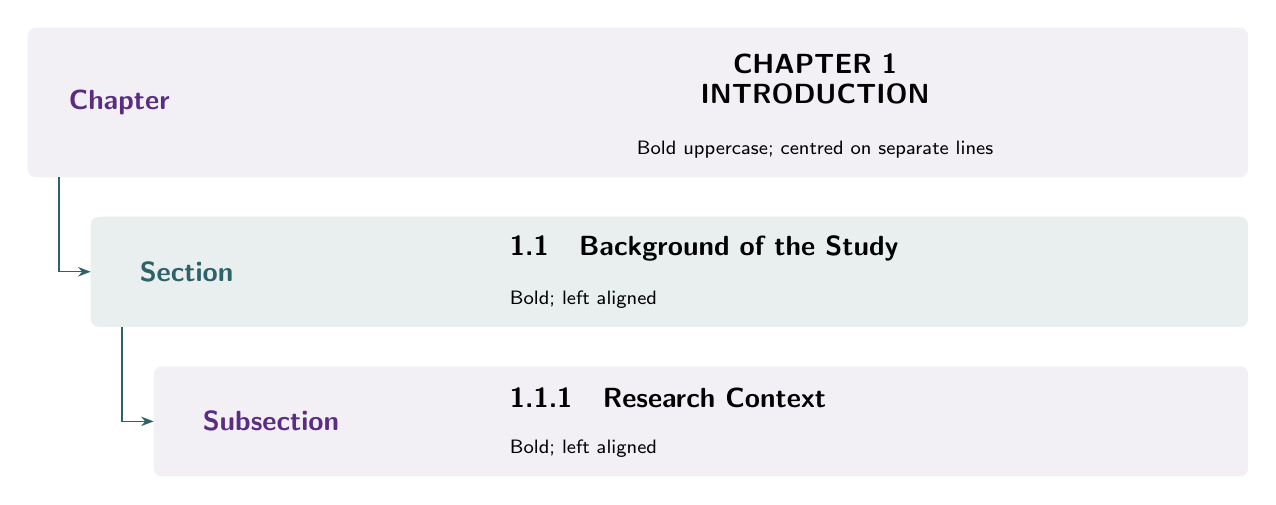
\begin{tikzpicture}[x=1mm,y=1mm,
  arr/.style={-{Stealth[length=1.6mm]},draw=iucteal,line width=0.5pt}]
  \fill[iuclav,rounded corners=3pt] (0,0) rectangle (155,-19);
  \node[anchor=west,font=\sffamily\bfseries\color{iucpurple}] at (4,-9.5) {Chapter};
  \node[font=\sffamily\bfseries,align=center] at (100,-6.5) {CHAPTER 1\\[-1pt]INTRODUCTION};
  \node[font=\sffamily\scriptsize] at (100,-15.5) {Bold uppercase; centred on separate lines};
  \fill[iuctealbg,rounded corners=3pt] (8,-24) rectangle (155,-38);
  \node[anchor=west,font=\sffamily\bfseries\color{iucteal}] at (13,-31) {Section};
  \node[anchor=west,font=\sffamily\bfseries] at (60,-28) {1.1\quad Background of the Study};
  \node[anchor=west,font=\sffamily\scriptsize] at (60,-34.5) {Bold; left aligned};
  \fill[iuclav,rounded corners=3pt] (16,-43) rectangle (155,-57);
  \node[anchor=west,font=\sffamily\bfseries\color{iucpurple}] at (21,-50) {Subsection};
  \node[anchor=west,font=\sffamily\bfseries] at (60,-47) {1.1.1\quad Research Context};
  \node[anchor=west,font=\sffamily\scriptsize] at (60,-53.5) {Bold; left aligned};
  \draw[arr] (4,-19) |- (8,-31);
  \draw[arr] (12,-38) |- (16,-50);
\end{tikzpicture}
\caption{Heading hierarchy and displayed alignment. Diagram indentation indicates hierarchy only.}
\label{fig:headings}
\end{figure}

Chapter, section, and subsection headings are bold and 12-point. Chapter headings
are uppercase and centred; sections and subsections are left aligned.

Use chapters, sections, and subsections only. Keep chapter titles uppercase, and
use title case for section and subsection headings. Set section and subsection
spacing to 24~pt before and 12~pt after. Leave 12~pt between the chapter
identifier and the chapter title, and 24~pt after the title.

\subsection{Capitalization and numbering}

Use uppercase chapter titles and title case for sections and subsections. Let
the template number headings consecutively. Match headings to the contents
entries, and do not end headings with a full stop.

% ===========================================================================
\section{Language and academic writing}
% ===========================================================================

Use clear, formal, grammatical language. Keep terminology, spelling,
capitalization, abbreviations, symbols, and units consistent.

Candidates should:

\begin{itemize}
  \item define specialist terms and uncommon abbreviations at first use;
  \item use one consistent variety of English unless another language is approved;
  \item keep names of variables, constructs, categories, and research
        instruments consistent;
  \item distinguish clearly between their own findings and claims from previous
        literature;
  \item avoid unsupported generalizations and informal expressions;
  \item present numbers, dates, percentages, and units consistently; and
  \item proofread both the text and the visual material after final pagination.
\end{itemize}

Check word counts using Section~\ref{sec:words}.

% ===========================================================================
\section{Tables}
% ===========================================================================

Use a table when rows and columns make information clearer. Introduce and
discuss each table in the text.

\subsection{Numbering and captions}

Number tables by chapter (for example, Table~4.1), and place the number and
caption above the table.

Write short, descriptive captions with consistent capitalization and
punctuation. Do not simply repeat the section heading.

Single-space captions, headings, data, and notes. Do not add blank lines or extra
spacing in rows or cells. Keep the surrounding body text double-spaced.

\subsection{Table design}

\begin{itemize}
  \item Use clear column headings, and include units where relevant.
  \item Single-space the whole table, without extra row spacing.
  \item Align comparable values, especially decimals.
  \item Avoid unnecessary gridlines.
  \item Explain abbreviations, symbols, statistical significance, and
        exceptions in table notes.
  \item Identify the source when a table is reproduced or adapted from another work.
  \item Obtain permission where required, and acknowledge the copyright holder.
  \item Keep text readable at the final print size.
\end{itemize}

Keep tables within the margins. For large tables, use landscape pages, split
them, repeat headings across pages, or move them to an appendix.

\keepwithsample
\textbf{Table example.} Introduce the table in the text and place its caption
above it.

\begin{figure}[H]
\panelhead{Table presentation}{Format notes}
\centering
\begin{tikzpicture}[x=1mm,y=1mm]
  \openpage{14}
  \fnote{1}{-8}{Page context}{This table is on a chapter-opening page, so the
    top margin is 40~mm.}{92.5,-20}
  \fnote{2}{-42}{Caption}{Number tables by chapter. Place the caption above the
    table.}{72.5,-46}
  \fnote{3}{-76}{Table and notes}{Single-space the caption, table, and notes.
    Keep them inside the text area.}{69,-60}
  \fnote{4}{-110}{Surrounding text}{Introduce and discuss the table in
    double-spaced body text.}{75,-66.5}
  \scalenote
\end{tikzpicture}
\caption{Table sample.}
\label{fig:tablesample}
\end{figure}

\clearpage
% ===========================================================================
\section{Figures}
% ===========================================================================

Figures include charts, diagrams, maps, photographs, and other visuals. Include
only figures that support the discussion, and refer to each one in the text.

\subsection{Numbering and captions}

Number figures by chapter (for example, Figure~4.1), and place the caption
below the figure.

Describe the figure briefly. Define unfamiliar symbols, colours, line styles,
and abbreviations in the caption or legend.

\subsection{Image quality}

\begin{itemize}
  \item Use images that are sharp at the final print size.
  \item Keep labels, axes, legends, and notes readable.
  \item Use colour when it improves clarity.
  \item Make graphs readable in greyscale where possible.
  \item Preserve image proportions.
  \item State the source of reproduced or adapted figures, and obtain
        permission where required.
\end{itemize}

Place each figure after its first mention or on the nearest suitable page. Keep
the figure and caption within the margins.

\keepwithsample
\textbf{Figure example.} Introduce the figure in the text, centre it, and place
its caption and source below it.

\begin{figure}[H]
\panelhead{Figure presentation}{Format notes}
\centering
\begin{tikzpicture}[x=1mm,y=1mm]
  \openpage{14}
  \fnote{1}{-8}{Artwork}{Keep axes, labels, and legends readable at the full
    printed size. Preserve proportions.}{78,-95}
  \fnote{2}{-42}{Caption and source}{Place the caption below the figure;
    single-space the caption and source note.}{77.5,-113}
  \fnote{3}{-76}{Cross-reference}{Refer to the figure by number in the
    text before it appears.}{81,-79.5}
  \fnote{4}{-110}{Surrounding text}{Discuss the figure in the double-spaced
    chapter text.}{71,-121.5}
  \scalenote
\end{tikzpicture}
\caption{Figure sample.}
\label{fig:figuresample}
\end{figure}

\clearpage
% ===========================================================================
\section{Equations, symbols, and units}
% ===========================================================================

Centre important displayed equations and number them by chapter, with the number
aligned at the right margin (for example, Equation~(3.1)).

Define symbols at first use. Use consistent type for variables, vectors,
matrices, functions, units, and labels, and punctuate equations as part of the
sentence.

Include every numbered equation in the list of equations with a short
descriptive title; do not reproduce the full expression in the list.

\keepwithsample
\textbf{Equation example.} Introduce the equation, number it by chapter, and
define its symbols.

\begin{figure}[H]
\panelhead{Equation presentation}{Format notes}
\centering
\begin{tikzpicture}[x=1mm,y=1mm]
  \openpage{13}
  \fnote{1}{-8}{Page context}{This equation is on a chapter-opening page with a
    40~mm top margin.}{92.5,-20}
  \fnote{2}{-42}{Equation}{Centre the expression; align its chapter-based
    number at the right margin.}{92.5,-49}
  \fnote{3}{-76}{Symbols}{Define symbols at first use, and use consistent
    mathematical typography.}{92.5,-57}
  \fnote{4}{-110}{Cross-reference}{Refer to the equation by number in the text,
    and include its short title in the list of equations.}{33,-66.5}
  \scalenote
\end{tikzpicture}
\caption{Equation sample.}
\label{fig:equationsample}
\end{figure}

\clearpage
% ===========================================================================
\section{Citations and references}
% ===========================================================================

Use APA 7th edition for all citations and references. Page layout, headings,
tables, and figure placement follow this manual. Author--year examples:

\begin{itemize}
  \item narrative: Lamport (1994) explains that \ldots;
  \item parenthetical: (Lamport, 1994); and
  \item multiple sources: (Knuth, 1984; Lamport, 1994).
\end{itemize}

Place \textbf{REFERENCES} after the chapters and before the appendices. Sort
entries alphabetically by first-author surname. Use 12-point Times New Roman,
double spacing, a 1.27~cm hanging indent, and no extra space between entries.

Check that:

\begin{itemize}
  \item every recoverable source cited in the text appears in the reference list;
  \item every reference-list entry is cited in the text;
  \item authors' names, publication dates, titles, editions, journal details,
        page ranges, and identifiers are accurate;
  \item capitalization and punctuation are consistent;
  \item direct quotations include the required page or location information;
  \item secondary citations are avoided or clearly identified; and
  \item APA 7th edition is applied consistently.
\end{itemize}

Check reference-manager and AI-generated output against the original sources.

Table~\ref{tab:cite} shows APA~7 citation forms. The sample sentences
illustrate formatting; they are not evidence for the claims shown.

\begin{table}[htbp]
\caption{Simulated author--year inline citation situations.}
\label{tab:cite}
\small
\begin{tabularx}{\textwidth}{@{}>{\raggedright\arraybackslash}p{38mm}X@{}}
\toprule
\thd{Situation} & \thd{Simulated text in the manuscript} \\
\midrule
Narrative, one author        & Lamport (1994) explains that document structure should remain consistent. \\
Parenthetical, one author    & Document structure should remain consistent (Lamport, 1994). \\
Narrative, two authors       & Creswell and Creswell (2018) describe several approaches to research design. \\
Parenthetical, two authors   & Several approaches may guide the research design (Creswell \& Creswell, 2018). \\
Three or more authors        & Devlin et al.\ (2019) introduced the model, which was later widely adopted. \\
Multiple sources             & Structured writing improves clarity and reproducibility (Knuth, 1984; Lamport, 1994). \\
Direct quotation             & Author (2024) states that ``clear structure supports careful reading'' (p.~18). \\
Specific page range          & The authors distinguish qualitative and quantitative designs (Creswell \& Creswell, 2018, pp.~3--5). \\
Same author, several years   & The framework developed across several studies (Smith, 2020, 2023). \\
Same author and year         & Both studies address the same population (Brown, 2022a, 2022b). \\
Group author, first use      & The guidance defines the required elements (American Psychological Association [APA], 2020). \\
Group author, later use      & The same guidance also addresses reference accuracy (APA, 2020). \\
Secondary citation           & Bandura's theory remains influential (Bandura, 1977, as cited in Smith, 2023). \\
Personal communication       & The revised procedure was confirmed by the programme office (A.~Rahman, personal communication, March~5, 2026). \\
Source without an author     & The formatting rules were subsequently revised (``Template Standards,'' 2024). \\
Source without a date        & The institutional guide emphasizes consistency (Innovative University College, n.d.). \\
\bottomrule
\end{tabularx}
\par\smallskip\raggedright\small\textit{Note.} Cite personal communications in
the text only. For secondary citations, list only the source actually read, and
use them sparingly. Section~\ref{sec:latexcite} gives the template command for
each situation.
\end{table}

\subsection{APA 7 reference rules}

\begin{itemize}
  \item Use surnames and initials. List all authors up to 20; for 21 or more,
        list the first 19, an ellipsis, and the final author.
  \item Use an ampersand before the final author in references and
        parenthetical citations, and \emph{and} in narrative citations.
  \item For three or more authors, use the first surname and \emph{et al.}\ in
        the text from the first citation, unless more names are needed to
        distinguish sources.
  \item Use sentence case for book, article, report, and webpage titles.
        Italicize standalone titles, journal names, and journal volume numbers;
        keep issue numbers in regular type.
  \item Include a DOI as a URL when available. Otherwise, include a URL for
        publicly accessible online sources, and omit routine academic-database
        URLs. Do not add a full stop after a DOI or URL.
  \item Omit the publisher or website name when it is the same as the author.
        Use \emph{n.d.}\ when no date is available. If there is no author, move
        the title to the author position.
  \item Order works by the same author from earliest to latest. Distinguish works
        by the same author in the same year with a, b, and so on, consistently
        in the text and references.
\end{itemize}

\textbf{Common reference patterns.} Replace the descriptive fields with the
source details. These are patterns, not sources to cite.

\begin{description}[style=nextline,leftmargin=1.2em,itemsep=3pt,font=\normalfont\bfseries]
  \item[Journal article] Author, A. A., \& Author, B. B. (Year). Article title.
    \emph{Journal Title, volume}(issue), page range. DOI or URL
  \item[Book] Author, A. A. (Year). \emph{Book title} (edition, if not the first).
    Publisher. DOI or URL
  \item[Edited-book chapter] Author, A. A. (Year). Chapter title. In E. E. Editor
    (Ed.), \emph{Book title} (pp.~xx--xx). Publisher. DOI or URL
  \item[Report] Organization. (Year). \emph{Report title} (Report No., if given).
    Publisher, if different from the author. URL
  \item[Webpage] Author or organization. (Year, Month Day). \emph{Page title}.
    Site name, if different from the author. URL
  \item[Thesis in a repository] Author, A. A. (Year). \emph{Thesis title}
    [Master's thesis or Doctoral dissertation, Institution]. Repository name. URL
\end{description}

\textbf{Quotations.} Enclose quotations of fewer than 40 words in quotation
marks. For 40 words or more, use a double-spaced block indented 1.27~cm from the
left, without quotation marks or extra space before or after. Give the author,
year, and page number; use a paragraph or section locator if the source has no
pages. Place a block quotation's citation after its closing punctuation.

\begin{figure}[H]
\panelhead{References}{Format notes}
\centering
\begin{tikzpicture}[x=1mm,y=1mm]
  \openpage{15}
  \fnote{1}{-8}{Heading}{REFERENCES: centred, bold uppercase, 12~pt.
    Chapter-opening margins.}{63.5,-21.5}
  \fnote{2}{-42}{Order}{APA~7; alphabetical by first-author surname.}{19.3,-42.6}
  \fnote{3}{-76}{Entries}{Times New Roman, 12~pt, double-spaced, with a
    1.27~cm hanging indent and no extra space between entries.}{25.5,-34.3}
  \fnote{4}{-110}{Pagination}{Continue Arabic numbering from the main
    chapters.}{57,-141}
  \scalenote
\end{tikzpicture}
\caption{References sample.}
\label{fig:refsample}
\end{figure}

\clearpage
% ===========================================================================
\section{Appendices}
% ===========================================================================

Use appendices for supporting material that would interrupt the chapters, such
as instruments, detailed tables, analyses, consent forms, interview guides, and
proofs.

Appendices follow the references and are identified alphabetically:

\begin{itemize}
  \item Appendix A: Research Instrument
  \item Appendix B: Supplementary Results
  \item Appendix C: Additional Documentation
\end{itemize}

Start each appendix on a new page with a descriptive title, and include it in
the contents and the list of appendices. Continue Arabic page numbering.

Refer to each appendix in the main text. Keep essential evidence and methods in
the relevant chapter.

\begin{figure}[H]
\panelhead{Appendix opening}{Format notes}
\centering
\begin{tikzpicture}[x=1mm,y=1mm]
  \openpage{16}
  \fnote{1}{-8}{Margins}{Use the chapter-opening layout: top 40~mm; other
    margins unchanged.}{92.5,-20}
  \fnote{2}{-42}{Identifier}{APPENDIX A, APPENDIX B, and so on, followed by a
    descriptive title.}{76,-27}
  \fnote{3}{-76}{Text}{Times New Roman, 12~pt. Double-spaced prose with 2~em
    indents and 6~pt after paragraphs.}{92.5,-37}
  \fnote{4}{-110}{Pagination}{Continue Arabic numbering through the
    appendices.}{56.5,-141}
  \scalenote
\end{tikzpicture}
\caption{Appendix-opening sample.}
\label{fig:appsample}
\end{figure}

% ===========================================================================
\section{Printing, paper, binding, and spine}
% ===========================================================================

These requirements apply to all study modes:

\begin{itemize}
  \item A4 white paper of at least 80~gsm, printed single-sided at actual size;
  \item black body text, with colour in figures and tables where it improves clarity;
  \item four final hardbound copies;
  \item purple covers and spines for all master's awards;
  \item black covers and spines for all doctoral awards, including professional doctorates;
  \item gold hot-stamped lettering in the sizes specified in this manual; and
  \item one final PDF; editable source files are not required.
\end{itemize}

There is no fixed PDF file-size limit. Use a clear filename that identifies the
student and the manuscript, for example \texttt{StudentID\_Surname\_Thesis.pdf}.
This naming pattern is recommended, not compulsory.

The PDF must open correctly, contain readable text and images, and match the
printed copies. Embed all fonts, and remove draft comments and tracked changes.
Check every page at its final size.

Match the cover and spine details to the title page and registration records.
Bind the final copies only after academic approval and a complete check of the
printed proof.

% ===========================================================================
% Section 18: Final manuscript review checklist (form page)
% ===========================================================================
\clearpage
\iucstripfalse
\thispagestyle{empty}
\refstepcounter{section}
\addcontentsline{toc}{section}{\protect\numberline{\thesection}Final manuscript review checklist}
\label{sec:checklist}
\newgeometry{top=16mm,bottom=16mm,left=20mm,right=20mm}
\begin{center}
  {\sffamily\bfseries\large INNOVATIVE UNIVERSITY COLLEGE\par}\vspace{6pt}
  {\sffamily\bfseries\Large FINAL MANUSCRIPT SUBMISSION CHECKLIST\par}\vspace{4pt}
  {\sffamily\small To be completed and returned with the manuscript\par}
\end{center}
\vspace{2pt}
\fcolorbox{iucpurple}{white}{\parbox{\dimexpr\textwidth-2\fboxsep-2\fboxrule}{\small
  \textbf{Formatting only; excludes academic content.} Complete the Student and
  Admin columns, sign below, and return this form with the manuscript.}}

\vspace{8pt}
{\large\bfseries Student and manuscript details\par}\vspace{4pt}
\renewcommand\arraystretch{1.9}
\begin{tabularx}{\textwidth}{@{}p{32mm}X p{25mm}p{32mm}@{}}
\textbf{Student name:} & \hrulefill & \textbf{Matric.\ no.:} & \hrulefill \\
\textbf{Programme:}    & \hrulefill & \textbf{Degree:}       & \hrulefill \\
\textbf{Faculty/unit:} & \hrulefill & & \\
\end{tabularx}
\begin{tabularx}{\textwidth}{@{}p{34mm}X@{}}
\textbf{Manuscript title:} & \hrulefill \\
\textbf{PDF filename:}     & \hrulefill \\
\textbf{Manuscript type:}  & \cbox~Thesis\qquad \cbox~Dissertation\qquad \cbox~Research project \\
\textbf{Submission stage:} & \cbox~Examination\qquad \cbox~Corrected final/deposit \\
\end{tabularx}
\renewcommand\arraystretch{1.2}

\vspace{6pt}
{\large\bfseries Template and formatting checklist\par}\vspace{3pt}
{\footnotesize
\begin{tabularx}{\textwidth}{@{}X>{\centering\arraybackslash}p{13mm}>{\centering\arraybackslash}p{13mm}@{}}
\toprule
\textbf{Review item} & \textbf{Student} & \textbf{Admin} \\
\midrule
A4 paper and the IUC page margins are used. & \cbox & \cbox \\
Body text uses Times New Roman 12~pt, double spacing, 2~em indents, and 6~pt after paragraphs. & \cbox & \cbox \\
Chapter and section headings follow the required format. & \cbox & \cbox \\
The compulsory minimum word count is met; both abstracts are included. & \cbox & \cbox \\
Front matter and Roman/Arabic page numbering are correct. & \cbox & \cbox \\
The table of contents and all lists match the manuscript. & \cbox & \cbox \\
Tables are single-spaced and use the required caption format. & \cbox & \cbox \\
Figures, equations, and appendices are numbered and formatted consistently. & \cbox & \cbox \\
Citations and references follow APA~7; references are double-spaced with hanging indents. & \cbox & \cbox \\
Every reference has been checked against its source, including any suggested by AI tools. & \cbox & \cbox \\
All text, tables, figures, and captions remain within the margins. & \cbox & \cbox \\
Placeholders, comments, draft marks, blank pages, and poor page breaks are removed. & \cbox & \cbox \\
The final PDF opens correctly; four hardbound copies meet the paper and cover rules. & \cbox & \cbox \\
\bottomrule
\end{tabularx}}

\vspace{8pt}
{\large\bfseries Final declaration and sign-off\par}\vspace{3pt}
The student and administrator confirm that formatting checks and required
corrections are complete.

\vspace{6pt}
\renewcommand\arraystretch{2.0}
\begin{tabularx}{\textwidth}{@{}p{38mm}X p{12mm}p{30mm}@{}}
\textbf{Student signature:}  & \hrulefill & \textbf{Date:} & \hrulefill \\
\textbf{Admin verification:} & \hrulefill & \textbf{Date:} & \hrulefill \\
\end{tabularx}
\renewcommand\arraystretch{1.2}
\restoregeometry
\clearpage
\iucstriptrue

% ===========================================================================
\section{Using the LaTeX template}\label{sec:latex}
% ===========================================================================

IUC provides a LaTeX template that applies Sections 2--17 automatically. It is
published, with its source and documentation, at \repo. This section explains
how to obtain it, how to work with it on your own computer, online, or with AI
tools, and which command produces each element of the manuscript.

\subsection{What the template does}

Candidates edit plain-text files: their details in \file{metadata.tex}, their
chapters in \file{chapters/}, and their sources in \file{references.bib}. The
template produces the PDF. Table~\ref{tab:map} shows how the rules in this
manual are applied.

\begin{table}[htbp]
\caption{How the template applies this manual.}
\label{tab:map}
\small
\begin{tabularx}{\textwidth}{@{}p{38mm}X>{\ttfamily\raggedright\arraybackslash}p{40mm}@{}}
\toprule
\thd{Rule (Section)} & \thd{Template behaviour} & \normalfont\thd{Command or file} \\
\midrule
Cover and title page (5)     & Generated from your details; white cover page in the PDF & metadata.tex \\
Front matter order (4, 6)    & Fixed order; empty lists omitted automatically           & main.tex \\
Margins, spacing (8)         & Applied automatically; 40~mm at chapter openings          & (automatic) \\
Page numbering (9)           & Roman i (hidden) to Arabic 1 at Chapter 1                 & \textbackslash mainmatter \\
Headings (10)                & Three levels; a fourth level stops the build              & \textbackslash chapter, \textbackslash section, \textbackslash subsection \\
Tables (12)                  & Numbered by chapter; caption above                       & \textbackslash caption, \textbackslash tablenote \\
Figures (13)                 & Numbered by chapter; caption below                       & \textbackslash caption, \textbackslash figuresource \\
Equations (14)               & Numbered by chapter; titled in the list                  & \textbackslash eqtitle \\
Citations, references (15)   & APA 7 via biblatex-apa                                   & \textbackslash parencite, references.bib \\
Appendices (16)              & APPENDIX A, B, \ldots; listed automatically              & \textbackslash appendix \\
Spine (5.1)                  & Spine strip for the binder                               & spine.tex \\
\bottomrule
\end{tabularx}
\par\smallskip\raggedright\small\textit{Note.} The template does not count words,
judge academic content, or check that references exist.
\end{table}

\subsection{Getting the template}

\textbf{Download.} On \repo, click \ui{Code}\then\ui{Download ZIP}. Use this for
Overleaf or your own computer.

\textbf{Your own repository.} Sign in to GitHub and open the template page.
\begin{enumerate}[itemsep=1pt,topsep=2pt]
  \item Click \ui{Use this template}\then\ui{Create a new repository}
        (or \ui{Fork} if that button is not shown).
  \item Name the repository, select \ui{Private}, and click \ui{Create repository}.
\end{enumerate} Use this for GitHub online and
Claude Code. Keep unpublished research, participant data, and passwords out of
any repository.

\begin{table}[htbp]
\caption{Contents of the template repository.}
\label{tab:files}
\small
\begin{tabularx}{\textwidth}{@{}>{\ttfamily}p{46mm}X>{\centering\arraybackslash}p{15mm}@{}}
\toprule
\normalfont\thd{File or folder} & \thd{Contents} & \thd{You edit} \\
\midrule
metadata.tex          & Title, name, matric number, address, degree, dates     & Yes \\
main.tex              & Order of the parts; document type on line~1             & Rarely \\
frontmatter/          & Acknowledgement, Abstrak, Abstract, optional pages     & Yes \\
chapters/             & \texttt{chapter1.tex} to \texttt{chapter5.tex}          & Yes \\
appendices/           & \texttt{appendixA.tex} and further appendices           & Yes \\
references.bib        & Reference entries in BibTeX format                     & Yes \\
figures/              & Images used in figures                                 & Yes \\
spine.tex             & Spine strip for the binder                             & No \\
iucthesis.cls         & The formatting rules                                   & No \\
latexmkrc, .vscode/, .github/ & Build settings                                 & No \\
\bottomrule
\end{tabularx}
\end{table}

\subsection{Choosing a workflow}

All workflows produce the same PDF (Table~\ref{tab:paths}).

\begin{table}[htbp]
\caption{Workflows for the template.}
\label{tab:paths}
\small
\begin{tabularx}{\textwidth}{@{}p{28mm}XXp{16mm}@{}}
\toprule
\thd{Workflow} & \thd{How it works} & \thd{Best for} & \thd{Install} \\
\midrule
Overleaf        & Edit and build in a web browser             & First-time LaTeX users             & Nothing \\
Own computer    & Free LaTeX system and an editor             & Long-term or offline work          & About 4 GB \\
GitHub online   & Edit on github.com; PDF built automatically & Backups, history, supervisor access & Nothing \\
AI assistant    & Describe changes; AI writes the LaTeX       & Anyone; combines with the others   & Nothing \\
\bottomrule
\end{tabularx}
\end{table}

\textbf{Overleaf.} Upload the ZIP with \ui{New Project}\then\ui{Upload Project}.
In \ui{Menu}, set \ui{Compiler} to \ui{XeLaTeX}, then click \ui{Recompile}. The
template has not yet been tested on Overleaf; confirm that the sample builds
before writing. Free accounts limit build time, which a long thesis with many
images can exceed.

\textbf{Own computer.} Install TeX Live (Windows, Linux) or MacTeX (macOS) from
\texttt{tug.org}. In Visual Studio Code, install the \textbf{LaTeX Workshop}
extension, open the template folder, and click \ui{Build LaTeX project}; the
included \file{.vscode/settings.json} selects XeLaTeX and biber. In TeXstudio,
set \ui{Default Compiler} to \ui{XeLaTeX} and \ui{Default Bibliography Tool} to
\ui{Biber}. From a terminal:

\begin{shell}
latexmk main.tex        # build main.pdf
latexmk spine.tex       # build spine.pdf for the binder
latexmk -c              # remove temporary files
\end{shell}

\textbf{GitHub online.} Edit a file with the pencil icon and click
\ui{Commit changes}. GitHub builds the PDF in about four minutes; download it
from \ui{Actions}\then latest run\then\textbf{Artifacts}. \ui{History} shows and
restores every earlier version, and \ui{Settings}\then\ui{Collaborators} gives a
supervisor access.

\textbf{Fonts.} Where Times New Roman and Arial Narrow are installed, the
template uses them. Otherwise it uses the metric-compatible TeX Gyre Termes and
TeX Gyre Heros Condensed, with the same layout. All fonts are embedded in the PDF.

\subsection{Entering your details and writing}

Enter your details once, in \file{metadata.tex}; they are reused on the cover,
title page, declaration, and spine. Replace only the text inside the braces.

\begin{code}
\title{Strategic Leadership and Organisational\\ Performance in Higher Education}
\author{Nur Aina Binti Rahman}             % full registered name
\matricno{IUC/PhD/2026/001}
\address{Kuala Lumpur, Malaysia}
\degree{Doctor of Philosophy in Management} % full degree name
\degreeabbr{PhD}                            % abbreviation for the spine
\submissiondate{October 2026}              % month and year
\submissionyear{2026}                      % year on the spine
\declarationdate{23 October 2026}
\end{code}

Line~1 of \file{main.tex} sets the document type: \texttt{thesis},
\texttt{dissertation}, or \texttt{project}. Write chapters in
\file{chapters/chapter1.tex} and the following files. A blank line starts a new
paragraph. Type \texttt{\textbackslash\%}, \texttt{\textbackslash\&},
\texttt{\textbackslash\$}, \texttt{\textbackslash\#}, and
\texttt{\textbackslash\_} to print those characters.

\begin{code}
\chapter{Literature Review}
\section{Leadership Theories}
\subsection{Transformational Leadership}

\begin{table}[htbp]
  \caption{Respondent Demographics}        % caption above the table
  \label{tab:demographics}
  \begin{tabular}{lcc}
    \toprule
    Group & Number & Percentage \\
    \midrule
    Male  & 120    & 48\% \\
    \bottomrule
  \end{tabular}
  \tablenote{Percentages are rounded.}
\end{table}

\begin{figure}[htbp]
  \includegraphics[width=0.8\textwidth]{figures/framework}
  \caption{Research Framework}             % caption below the figure
  \figuresource{Adapted from Smith (2023).}
\end{figure}

\begin{equation}
  y = \beta_0 + \beta_1 x + \varepsilon
  \eqtitle{Linear Regression Model}        % title in the list of equations
\end{equation}
\end{code}

To refer to a numbered item, give it a \cmd{label} and cite it with
\cmd{ref}, for example
\texttt{Table\textasciitilde\textbackslash ref\{tab:demographics\}}. After
\cmd{appendix} in \file{main.tex}, each \cmd{chapter} becomes an appendix.

\subsection{Citations in the template}\label{sec:latexcite}

Each source is an entry in \file{references.bib}; Google Scholar, Zotero,
Mendeley, and EndNote export this format. Cite the entry's key.
Table~\ref{tab:latexcite} gives the commands for the situations in
Table~\ref{tab:cite}, with the output produced by the template.

\begin{table}[htbp]
\caption{Citation commands and the output they produce.}
\label{tab:latexcite}
\small
\begin{tabularx}{\textwidth}{@{}>{\raggedright\arraybackslash}p{27mm}>{\ttfamily\raggedright\arraybackslash}p{66mm}>{\raggedright\arraybackslash}X@{}}
\toprule
\thd{Situation} & \normalfont\thd{Command} & \thd{Output} \\
\midrule
Narrative                    & \textbackslash textcite\{lamport1994\}            & Lamport (1994) \\
Parenthetical                & \textbackslash parencite\{lamport1994\}           & (Lamport, 1994) \\
Two authors                  & \textbackslash parencite\{creswell2018\}          & (Creswell \& Creswell, 2018) \\
Three or more authors        & \textbackslash textcite\{devlin2019\}             & Devlin et al.\ (2019) \\
Multiple sources             & \textbackslash parencite\{lamport1994,knuth1984\} & (Knuth, 1984; Lamport, 1994) \\
Page                         & \textbackslash parencite[p.\textasciitilde 18]\{lamport1994\} & (Lamport, 1994, p.~18) \\
Page range                   & \textbackslash parencite[pp.\textasciitilde 3-{}-5]\{creswell2018\} & (Creswell \& Creswell, 2018, pp.~3--5) \\
Same author, several years   & \textbackslash parencite\{smith2020,smith2023\}   & (Smith, 2020, 2023) \\
Same author and year         & \textbackslash parencite\{brown2022a,brown2022b\} & (Brown, 2022a, 2022b) \\
Group author                 & \textbackslash parencite\{apa2020\}               & First (American Psychological Association [APA], 2020); later (APA, 2020) \\
Secondary source             & \textbackslash parencite[Bandura, 1977, as cited in][]\{smith2023\} & (Bandura, 1977, as cited in Smith, 2023) \\
No author                    & \textbackslash parencite\{standards2024\}         & (``Template Standards,'' 2024) \\
No date                      & \textbackslash parencite\{iucguide\}              & (Innovative University College, n.d.) \\
\bottomrule
\end{tabularx}
\par\smallskip\raggedright\small\textit{Note.} The letters a and b, the
abbreviation in brackets (from the entry's \texttt{shortauthor} field), and n.d.\
are added automatically. Personal communications are typed directly in the text.
\end{table}

The template sets titles in sentence case, so put proper nouns and acronyms in
braces, for example \texttt{\{Malaysian\}} or \texttt{\{BERT\}}, and group
authors in double braces, for example
\texttt{\{\{Ministry of Education Malaysia\}\}}. Check every exported entry
against its source.

\subsection{Working with AI tools}

AI assistants can write and correct LaTeX. Table~\ref{tab:ai} compares three
ways to use them.

\begin{table}[htbp]
\caption{AI tools for the template.}
\label{tab:ai}
\small
\begin{tabularx}{\textwidth}{@{}p{26mm}XXp{15mm}@{}}
\toprule
\thd{Tool} & \thd{What the AI does} & \thd{What you do} & \thd{Builds PDF} \\
\midrule
Claude Code     & Edits the repository, builds and checks the PDF, saves the changes & Describe changes in plain words & Yes \\
Claude Projects & Drafts LaTeX with the template and this manual as context          & Paste answers into your files    & No \\
Any AI chat     & Answers one request at a time                                      & Paste text in; copy LaTeX out    & No \\
\bottomrule
\end{tabularx}
\end{table}

\textbf{Claude Code.} Open \texttt{claude.ai/code}, connect GitHub, start a
session on your thesis repository, and describe the change. Ask Claude to commit
and push the result.

\begin{promptbox}{Example requests}
Put my details in metadata.tex: title \ldots, name \ldots, matric number \ldots,
Master of Business Administration, submitted March 2027.\par
Add the attached survey results to Chapter 4 as a table captioned Respondent
Demographics.\par
Build the PDF and show me the contents page.
\end{promptbox}

\textbf{Claude Projects.} Create a project, add the repository under
\textbf{Project knowledge}\then\ui{GitHub}, upload this manual, and paste these
instructions. Click \ui{Sync} after changing files on GitHub.

\begin{prompttext}
I am writing an IUC thesis with the iucthesis LaTeX template in this project.
- Follow the IUC Style Manual and the template README.
- Use only \chapter, \section, and \subsection.
- Tables: \caption above the table; \tablenote{} for notes.
- Figures: \caption below the figure; \figuresource{} for the source.
- Every numbered equation needs \eqtitle{Short title}.
- Cite with \textcite{} or \parencite{} (APA 7); give BibTeX for new sources.
- Return LaTeX that I can paste straight into my chapter files.
\end{prompttext}

\textbf{Any AI chat assistant.} Claude, ChatGPT, Gemini, and Copilot all help
with single tasks. State that you use the IUC \emph{iucthesis} LaTeX template,
then ask, for example, to convert Word text to LaTeX, turn data into a table
with a caption and \cmd{tablenote}, create BibTeX entries with protected
capitals, or explain a build error.

\begin{warnbox}[Responsible use]
Candidates are responsible for everything in their thesis. AI tools can invent
sources, so verify every reference in the original publication or database.
Follow your programme's rules on AI use, including any requirement to declare
it. Do not give participant data, unpublished results, or personal information
to AI tools unless your ethics approval allows it.
\end{warnbox}

\subsection{Building, checking, and troubleshooting}

Page numbers, contents, lists, and cross-references update on the following
build; \texttt{latexmk}, Overleaf, VS Code, and GitHub repeat builds as needed.
Add \texttt{showframe} to line~1 of \file{main.tex} to draw the text area while
checking margins, and remove it before submission. Build \file{spine.tex} for
the binder's spine strip (Figure~\ref{fig:spine}).

LaTeX stops at the first serious error and prints a message beginning with
\texttt{!}. Table~\ref{tab:trouble} lists common causes.

\begin{table}[htbp]
\caption{Common error messages and their fixes.}
\label{tab:trouble}
\small
\begin{tabularx}{\textwidth}{@{}>{\raggedright\arraybackslash}p{46mm}>{\raggedright\arraybackslash}X>{\raggedright\arraybackslash}X@{}}
\toprule
\thd{Message or symptom} & \thd{Usual cause} & \thd{Fix} \\
\midrule
\texttt{This class needs XeLaTeX} & pdfLaTeX selected & Select XeLaTeX \\
\texttt{Missing \$ inserted} & \texttt{\_} or \texttt{\^{}} in normal text & Type \texttt{\textbackslash\_} or \texttt{\textbackslash\^{}\{\}} \\
Rest of a line missing & \texttt{\%} begins a comment & Type \texttt{\textbackslash\%} \\
\texttt{Missing \}} or \texttt{Runaway argument} & An unclosed \texttt{\{} & Close the brace \\
\texttt{Undefined control sequence} & Misspelt command & Check the spelling after \texttt{\textbackslash} \\
\texttt{Citation `\ldots' undefined} & Key not in \file{references.bib} & Check the key; build again \\
\texttt{??} instead of a number & Not yet updated & Build again \\
\texttt{\textbackslash subsubsection is not permitted} & A fourth heading level & Use \cmd{subsection} \\
Title printed in lowercase & Unprotected capitals in \file{.bib} & Put the word in braces \\
\bottomrule
\end{tabularx}
\end{table}

Undo the most recent change and build again to isolate a problem. Report
template faults on the template's GitHub page under \ui{Issues}.

% ===========================================================================
% Back cover
% ===========================================================================
\clearpage
\iucstripfalse

\includepdf[pages=1]{cover-back}

\end{document}
